\section{Setting and notation}\label{sec:setting}

\subsection{Fibres of occurrence sets}
A \emph{state} is a positive rational $x=a/b$ in lowest terms. Its occurrence set is $D(x)=\{d\ge2: d^2\mid a,\ d\equiv1\ (\mathrm{mod}\ b)\}$ (Foundations Vol.~I, Thm.~1.2~\cite{FoundI}). Let $\Pcal=\{p_1<\dots<p_k\}$ be the primes with $p_i^2\mid a$, $q_i=\lfloor v_{p_i}(a)/2\rfloor\ge1$, and $Q=\prod_{i}[0,q_i]$ the \emph{box}. For $\alpha\in\Z^k$ put $\chi_b(\alpha)=\prod_i p_i^{\alpha_i}\bmod b$ (negative exponents through inverses; $\gcd(p_i,b)=1$ because $\gcd(a,b)=1$) and
\[
\Lambda_b=\ker\chi_b\subseteq\Z^k,\qquad F(\Lambda,Q)=(\Lambda\cap Q)\setminus\{0\}.
\]
\begin{proposition}[fibre]\label{prop:fibre}
The map $\alpha\mapsto\prod p_i^{\alpha_i}$ is a bijection $F(\Lambda_b,Q)\to D(x)$. The index is $[\Z^k:\Lambda_b]=|H_b|$ with $H_b=\langle p_1,\dots,p_k\rangle\le(\Z/b)^\times$.
\end{proposition}
\begin{proof}
If $d^2\mid a$ then every prime factor $p$ of $d$ has $p^2\mid a$, so $d=\prod p_i^{\alpha_i}$ with $0\le\alpha_i\le q_i$; this exponent vector is unique, and $d\equiv1\pmod b$ iff $\chi_b(\alpha)=1$. The vector $\alpha=0$ gives $d=1\notin D(x)$. The map $\chi_b:\Z^k\to H_b$ is onto with kernel $\Lambda_b$. \qedhere
\end{proof}
For $b=1$ we have $\Lambda_1=\Z^k$. A lattice here always means a full-rank sublattice of $\Z^k$ (finite index); this holds for every $\Lambda_b$.

\subsection{Moves, cells and the three objects}
\begin{definition}[conformal order, Graver set]
For $v,w\in\Z^k$ write $w\cm v$ if $w_iv_i\ge0$ and $|w_i|\le|v_i|$ for all $i$. For a lattice $\Lambda$, $\Gr(\Lambda)$ is the set of $\cm$-minimal nonzero elements of $\Lambda$ (the \emph{Graver set}); it is symmetric under $v\mapsto-v$ (Graver~\cite{Graver1975}; see also \cite{Sturmfels1996,DLHK2013}). For $q\in\Z_{>0}^k$ the \emph{region Graver set} $\Gr_q(\Lambda)$ is the set of $\cm$-minimal nonzero elements of $\Lambda\cap[-q,q]$.
\end{definition}
\begin{definition}[cell]\label{def:cell}
Let $g_1,\dots,g_j\in\Gr_q(\Lambda)$ be linearly independent and $u\in\Z^k$. The parallelotope $\Pil(u;g_1,\dots,g_j)=u+\sum_i[0,1]g_i$ is a \emph{$j$-cell of $(\Lambda,Q)$} if all its $2^j$ corners lie in $F(\Lambda,Q)$. (A $0$-cell is a point of $F$.) The \emph{abstract complex} $\Kabs(\Lambda,Q)$ is the set of all cells, a cell being identified with its vertex set (\cref{lem:intrinsic}); it is closed under taking faces. The \emph{realised union} is $U(\Lambda,Q)=\bigcup$ of the closed cells. The \emph{origin-allowed union} $U^0(\Lambda,Q)$ is defined in the same way with the corners allowed to be $0$.
\end{definition}
The origin is excluded because $\alpha=0$ corresponds to $d=1\notin D(x)$. This single exclusion is the source of every phenomenon in this manuscript. A third object, the \emph{embedded subdivision} $\Kemb$, exists only when any two closed cells meet in a common face; it is never needed below and when a statement is about $\Kabs$, $U$ or $\Kemb$ it says so. Boundaries of cells in $\Kabs$ are $\partial\Pil(u;g_1..g_j)=\sum_i(-1)^{i-1}[\Pil(u+g_i;\widehat{g_i})-\Pil(u;\widehat{g_i})]$; $\partial\partial=0$.

\begin{lemma}[cells are intrinsic]\label{lem:intrinsic}
Order $\Z^k$ lexicographically. A cell $c$ with vertex set $V(c)$ has its lexicographically smallest vertex $m(c)$ as a base point and the set $\mathrm{Gen}(c)$ of its generators, taken lexicographically positive, equals the set of edge vectors of $\conv V(c)$ at $m(c)$. In particular $V(c)$ determines $c$ and $\mathrm{Gen}(c)$.
\end{lemma}
\begin{proof}
$\conv V(c)=\Pil(u;g_1..g_j)$ is a $j$-dimensional parallelotope; its vertices are $u+\sum_{i\in S}g_i$. The lexicographic order is translation invariant, so the smallest vertex is $u+\sum_{g_i<0}g_i$, and the edges at that vertex of the parallelotope are along $\pm g_i$ leaving in the lexicographically positive direction. Edges of $\conv V(c)$ depend only on the convex body, hence only on $V(c)$. \qedhere
\end{proof}
Remark: since $\Gr_q(\Lambda)=-\Gr_q(\Lambda)$, ``$\mathrm{Gen}(c)\subseteq\Gr_q(\Lambda)$'' does not depend on orientations.
\begin{figure}[tbp]\centering
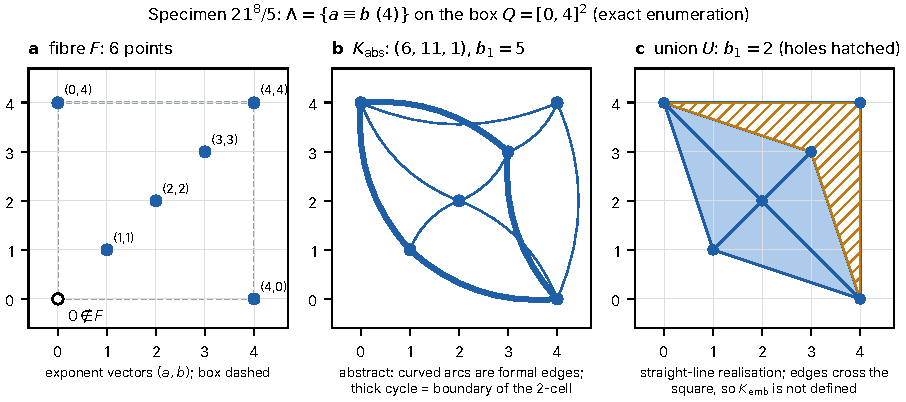
\includegraphics[width=0.98\textwidth]{fig01_three_objects}
\caption{The three objects for the specimen $21^8/5$ ($\Lambda=\{a\equiv b\ (4)\}$, $Q=[0,4]^2$; \emph{exact computation}). (a)~The fibre $F(\Lambda,Q)$: six points, the origin being excluded. (b)~The abstract complex $\Kabs$: f-vector $(6,11,1)$, Betti numbers $(1,5,0)$; edges are drawn as arcs to stress that they are formal incidences, and the thick cycle bounds the single $2$-cell. (c)~The realised union $U$ of the closed cells with straight edges: it has two bounded complementary components (hatched), so $b_1(U)=2\ne b_1(\Kabs)=5$. Edges of $\Kabs$ cross inside the square, so closed cells do not all meet in common faces and $\Kemb$ is \emph{not} defined for this specimen. The Betti numbers agree with those reported by the release; $b_1(U)$ was obtained here with a floating-point polygon routine on exact integer coordinates (\cref{def:cell}, \cref{prop:topology}).}\label{fig:objects}
\end{figure}

\subsection{Notation table}
\begin{center}\small
\begin{tabular}{@{}p{0.30\textwidth}p{0.64\textwidth}@{}}\toprule
symbol & meaning\\\midrule
$x=a/b$; $D(x)$ & state; occurrence set\\
$\Pcal=\{p_i\}$, $Q=\prod[0,q_i]$ & active primes; exponent box\\
$\Lambda_b$, $H_b$, $\chi_b$ & relation lattice, group generated by the primes mod $b$, character\\
$F(\Lambda,Q)$ & fibre $(\Lambda\cap Q)\setminus\{0\}$\\
$\Gr(\Lambda)$, $\Gr_q(\Lambda)$ & Graver set; region Graver set (the source writes $G$; $G$ is also the gcd of FIELD-I)\\
$\cm$ & conformal order\\
$\Pil(u;g_1..g_j)$, $\Kabs$, $U$, $U^0$ & cell (source: $P(u;\dots)$), abstract complex, union, origin-allowed union\\
$E_k$ & even-sum lattice $\{z\in\Z^k:\sum z_i\text{ even}\}$ (index $2$)\\
$\Cmap$ & collective map $x\mapsto x+L^2/G$ with $L=\mathrm{lcm}\,D(x)$, $G=\gcd\{d-1\}$\\
$v^+,v^-$ & $\max(v,0)$, $\min(v,0)$ coordinatewise\\\bottomrule
\end{tabular}
\end{center}

\subsection{Model boundaries}
The objects here belong to the model classes M7 (lattice and target transport) and, for the arithmetic inputs, M1 (FIELD-I collective map) and M2/M3 (GEO-I occurrence geometry, planar model). The binary $0/1$ obstruction model (M4), the rational-state move complexes $K_{\mathrm{axis}},K_{\mathrm{move}}$ (M5) and the history complexes (M6) are different objects and are not used. The map $\Cmap$ is one specified collective rule; it is not forced by the arithmetic formula for $D(x)$. A \emph{transition} $x\to x'=\Cmap(x)$ is called \emph{admissible} if $x'$ has the same active primes and box; only admissible transitions are compared here.
